\documentclass[conference]{IEEEtran}
\IEEEoverridecommandlockouts

\usepackage{cite}
\usepackage{amsmath,amssymb,amsfonts}
\usepackage{algorithmic}
\usepackage{graphicx}
\usepackage{textcomp}
\usepackage{xcolor}
\usepackage{booktabs}
\usepackage{multirow}
\usepackage{url}

\newcommand{\bench}{EviStateBench}
\newcommand{\engine}{EviStateDB}
\newcommand{\tsv}{TemporalStateView}
\begin{document}

\title{[Experiment, Analysis, and Benchmark] EviStateBench: Evaluating Temporal Task-State View Maintenance over Embodied Observation Streams}

\author{\IEEEauthorblockN{Anonymous Authors}
\IEEEauthorblockA{Paper under submission}}

\maketitle

\begin{abstract}
Embodied agents increasingly produce streams of observations from perception modules, action logs, trackers, task monitors, and simulators. These streams are noisy, delayed, out of order, incomplete, and sometimes contradictory, yet downstream task execution often needs an auditable view of task state: whether an object is inside a container, whether a device is open or toggled on, whether a goal predicate currently holds, and how that answer changes under late evidence. Existing embodied benchmarks emphasize task completion, navigation, question answering, or memory recall; they do not isolate the data-management problem of maintaining temporal task-state views from imperfect observation streams.

We introduce \bench, an Experiment, Analysis, and Benchmark contribution for temporal task-state view maintenance over embodied observation streams. \bench\ derives hidden state timelines from simulator truth and task specifications, emits public StateObservation streams, provides workloads for bitemporal state, provenance, change-set, uncertainty, precondition, failure-localization, and goal queries, and evaluates predicted answers against hidden answer sets. The reported artifact contains 570 simulator-grounded episodes over 36 activities, 5,848 hard queries, 2.86M clean observations, and 2.80M hard mixed observations, with public-artifact, query-semantics, and answer-schema validation passing without errors. We also provide \engine, a reference baseline engine that maintains bitemporal task-state views with support and contradict evidence. Experiments with recall-memory, temporal-log, and \engine\ baselines show that the benchmark separates retrieval memory, temporal-log lookup, and materialized temporal-state maintenance: exact accuracy ranges from 25.2\% to 75.6\%, while structured, set-valued, and task-derived queries remain challenging.
\end{abstract}

\begin{IEEEkeywords}
benchmarking, temporal data management, stream processing, embodied AI, task state, provenance, uncertain data
\end{IEEEkeywords}

\section{Introduction}

Embodied agents observe the world through imperfect streams. A robot may receive a detector output that a cabinet is open, a relation estimate that a cup is inside the cabinet, an action log that a place operation succeeded, and a later visual observation that appears to contradict the earlier relation. These observations arrive from different sources, at different times, and with different reliability. Some refer to the current world state; others arrive late and describe an earlier event. Some are missing because an object was occluded. Some are wrong because perception failed. A task executor nevertheless needs to ask database-like questions: does the goal hold now, what did the agent know at a previous transaction time, which state changed during the episode, and which evidence supports or contradicts an answer?

Current embodied benchmarks and simulators provide important foundations, but they do not directly evaluate this maintenance problem. BEHAVIOR describes household activities with predicate-logic initial and goal conditions~\cite{srivastava2022behavior}, and BEHAVIOR-1K extends the scale and simulation environment for long-horizon mobile manipulation~\cite{li2024behavior1k}. Habitat, AI2-THOR, VirtualHome, and TEACh provide embodied environments, task programs, rearrangement, or interactive instruction-following settings~\cite{savva2019habitat,szot2021habitat,kolve2017ai2thor,puig2018virtualhome,padmakumar2022teach}. OpenEQA evaluates open-vocabulary embodied question answering over episodic memory and active exploration~\cite{majumdar2024openeqa}. ALFRED evaluates grounded instruction following for everyday tasks~\cite{shridhar2020alfred}. These benchmarks expose task, language, perception, and interaction challenges, but the primary scoring target is not whether a data system can maintain a temporal task-state view with valid-time semantics, transaction-time repair, provenance, and query workloads over public observation streams.

This distinction matters for data engineering. In a task such as placing a cup into a cabinet and closing the door, the relevant maintained states may include \texttt{inside(cup,cabinet)}, \texttt{open(cabinet)}, and \texttt{grasped(robot,cup)}. The query \emph{was the cup inside the cabinet after the place action?} is not a retrieval query over similar frames. It is a temporal state query over evidence. The query \emph{what changed between the beginning and end of the episode?} is not a single symbolic-state lookup. It is a state-diff query over a maintained view. The query \emph{would the system have known this before the delayed observation arrived?} requires event time and arrival time to be separated. These requirements connect embodied observation streams to temporal databases, stream processing, incremental view maintenance, uncertain data, and provenance~\cite{snodgrass1999developing,jensen1999temporal,babcock2002models,gupta1995maintenance,zhuge1995view,aggarwal2009uncertain,green2007provenance,cheney2009provenance}.

We introduce \bench, a data-management benchmark for evaluating temporal task-state view maintenance over embodied observation streams. A \bench\ task instance provides public inputs, including task specifications, observation streams, queries, and metadata. It withholds hidden timelines and answer sets used by the evaluator. Systems under test may use any internal representation: retrieval memory, temporal logs, SQL scans, rules, materialized views, learned memory, or a hybrid. They are compared only by their predicted query answers under a shared evaluator. This public/hidden split is central: the oracle is derived from simulator truth and task specifications, not from any submitted system.

We also provide \engine, a reference baseline engine. \engine\ maintains a \tsv\ with valid-time intervals, transaction-time revisions, support and contradict evidence, confidence, and task-derived views. It is useful for diagnosing what a temporal view-maintenance engine can do under the benchmark, but it is not the benchmark oracle. This separation lets \bench\ evaluate \engine\ alongside simpler baselines such as latest observation, temporal-log scan, SQL scan, and retrieval-style memory.

This paper makes four contributions.
\begin{itemize}
    \item We formulate temporal task-state view maintenance over embodied observation streams as a data-management benchmark problem.
    \item We define the \bench\ artifact boundary, observation schema, query workloads, perturbation regimes, answer schema, and evaluator semantics.
    \item We describe a simulator-grounded generator that produces hidden state timelines, clean and perturbed public observation streams, query sets, hidden answer sets, and validation reports.
    \item We provide \engine\ as a reference baseline engine and define an experimental protocol for comparing systems under shared public inputs and hidden oracle answers.
\end{itemize}

The intended EAB contribution is therefore not a new perception model, planner, or robotics controller. It is the benchmark object: a standardized artifact, a query workload, an evaluator, a public/hidden boundary, and an analysis protocol for systems that maintain temporal task-state views. This mirrors database benchmark and EAB papers that introduce evaluation frameworks and diagnostic workloads to expose trade-offs that are hard to see in one-off experiments~\cite{erling2015ldbc,iosup2016ldbc,khelifati2023tsmbench,qi2025finbench,malekpour2026sqlmorph,najafi2025beacon,mu2025aqp}.

\section{Motivation and Benchmark Scope}
\label{sec:motivation}

\subsection{A Running Task-State Example}

Consider a household task in which an agent must put a cup in a cabinet and close the cabinet. The task is naturally described by predicates over objects and time: the cup should be inside the cabinet, the cabinet should eventually be closed, and the robot should no longer be grasping the cup. A simulator or action script can provide the hidden state changes, but a deployed system observes a stream of partial evidence. A relation detector may report \texttt{inside(cup,cabinet)} with moderate confidence after the place action. A visual detector may miss the cup after it becomes occluded. An action log may assert that the place action succeeded. A later observation may arrive after the close action and repair an earlier belief.

This example separates three notions that are often collapsed. First, \emph{world state} is what actually holds in the simulator at a valid time. Second, \emph{observation evidence} is what a source claims, possibly late or incorrectly. Third, \emph{maintained task-state view} is what a system can answer after ingesting the public stream. \bench\ evaluates the third object against hidden answers derived from the first object, using only the second object as public input.

\subsection{What the Benchmark Evaluates}

\bench\ evaluates systems that maintain queryable temporal views of task state. A system is given a task specification, an observation stream, and a query set. It outputs predicted answers. The evaluator checks those answers against hidden answer sets. The system is not required to expose its internal state view; it may implement a log scan, a materialized view, a database table, a retrieval index, or a learned model. The only required output is the standardized predicted QueryAnswer.

The benchmark focuses on eight query families. \texttt{AS\_OF\_STATE} asks what would be known for a valid time at a specified transaction time. \texttt{WHY\_STATE} asks which evidence supports the maintained state. \texttt{STATE\_DIFF} asks which states changed between two valid-time points or intervals. \texttt{FIND\_UNCERTAIN\_STATES}, \texttt{CHECK\_PRECONDITION}, and \texttt{FAILURE\_LOCALIZATION} expose set-valued uncertainty, task-precondition, and failure-analysis views. \texttt{CHECK\_STATE} and \texttt{CHECK\_GOAL} provide compact point-state and goal-state probes.

\subsection{What the Benchmark Deliberately Excludes}

\bench\ is not a robot-control benchmark. It does not score low-level manipulation success, exploration policy, path planning, or visual perception quality as primary outcomes. Those components are important, but mixing them into the main benchmark would make it difficult to attribute failures to temporal state-view maintenance. The main artifact therefore uses simulator-grounded hidden timelines and controlled public observation streams. Action-source and perception-source gaps are stated as scope limits; the main correctness claims are made over the controlled data-management workload.

This scope is intentionally narrow. A benchmark for view maintenance must make the stream, queries, hidden answers, and evaluation semantics stable. Otherwise, an accuracy difference may reflect perception quality, controller robustness, simulator physics, or task policy rather than the state-maintenance method being evaluated. \bench\ isolates the data-management layer so that systems can compare maintenance strategies under the same public inputs.

\subsection{Benchmark Requirements}

The running example gives rise to five benchmark requirements. \emph{R1: temporal semantics.} The benchmark must ask about both current and historical task states, not only final task success. \emph{R2: information availability.} It must separate valid time from arrival time so that late evidence can repair a previous state without pretending that the system knew it earlier. \emph{R3: evidence sensitivity.} It must include support and contradict observations because task states can become uncertain or conflicting. \emph{R4: task-derived views.} It must evaluate predicates in the context of task goals, not only isolated object attributes. \emph{R5: reproducibility.} It must provide public inputs, hidden answers, validation reports, and a shared evaluator.

Table~\ref{tab:related-benchmarks} positions these requirements against related benchmark families. The point is not that prior benchmarks are deficient for their own goals; rather, they target different layers of the embodied stack. \bench\ fills the data-management layer between observation-producing embodied systems and task executors that need queryable, auditable state.

\begin{table*}[!t]
\caption{Benchmark positioning. Related embodied benchmarks provide task, simulation, language, or memory-recall evaluation, while \bench\ isolates temporal task-state view maintenance.}
\label{tab:related-benchmarks}
\centering
\scriptsize
{\setlength{\tabcolsep}{2pt}
\begin{tabular}{@{}p{0.13\textwidth}p{0.16\textwidth}p{0.11\textwidth}p{0.11\textwidth}p{0.12\textwidth}p{0.11\textwidth}p{0.10\textwidth}@{}}
\toprule
Benchmark family & Primary target & Temporal state queries & Event/arrival time & Perturbed observations & Task-derived views & Hidden oracle \\
\midrule
BEHAVIOR / BEHAVIOR-1K & Household task execution and simulation & Partial & No & No & Goal predicates & Simulator truth \\
ALFRED & Instruction following & No & No & No & Task success & Demo labels \\
OpenEQA & Embodied question answering & Episodic context & No & No & NL answers & Human/LLM scoring \\
Retrieval memory evals & Recall from stored observations & Limited & No & Usually no & No & Dataset labels \\
\bench & Temporal task-state view maintenance & Yes & Yes & Yes & Yes & Simulator truth + specs \\
\bottomrule
\end{tabular}
}
\end{table*}

\section{Problem Definition}
\label{sec:problem}

\subsection{Episodes, Task Specifications, and Hidden Timelines}

An episode $e$ is an execution instance of a task specification. A task specification defines objects, predicates, initial conditions, goal conditions, and task-level metadata. Let $\mathcal{P}$ be the set of task-state predicates, such as \texttt{open}, \texttt{inside}, \texttt{toggled\_on}, \texttt{covered}, \texttt{cooked}, \texttt{temperature}, \texttt{frozen}, and \texttt{attached}. A state atom has the form $p(\mathbf{a})=v$, where $p\in\mathcal{P}$, $\mathbf{a}$ is a tuple of object identifiers or values, and $v$ is a Boolean, categorical, or numeric value.

For each episode, the generator constructs a hidden state timeline
\begin{equation}
    H_e = \langle h_1,\ldots,h_m\rangle,
\end{equation}
where each event $h_i$ records a state atom, a value, and a valid-time interval or transition time derived from simulator truth and task specifications. Hidden timelines are not part of the public input. They are used to generate hidden answer sets.

\subsection{StateObservation Streams}

The public input stream is a sequence of StateObservations. Each observation is a tuple
\begin{equation}
\begin{split}
o = (&obs\_id, episode\_id, event\_time, arrival\_time, source,\\
     &kind, predicate, arguments, value, confidence,\\
     &polarity, evidence\_ref, metadata).
\end{split}
\end{equation}
The \emph{event time} is the time to which the observation refers in the episode. The \emph{arrival time} is the time at which the system receives the observation. The two may differ, which creates the need for transaction-time semantics. The \emph{polarity} indicates whether the observation supports, contradicts, or corrects a state claim. The \emph{evidence reference} links to the evidence item in the artifact, such as a frame identifier, trajectory identifier, source record, or simulator-derived annotation.

An observation stream can be clean or perturbed. Clean streams reflect simulator-derived observations with minimal injected noise. Perturbed streams inject missing observations, temporal disorder, low confidence, and contradictions. The reported release includes a target-aware hard mixed stream that combines several issues and acts as the primary stress test.

The distinction between event time and arrival time is central. If an observation with $event\_time=10$ arrives at $arrival\_time=40$, then a system answering at transaction time 20 should not be credited for using it, while a system answering at transaction time 50 may use it to repair the maintained view. This is the benchmark analogue of bitemporal data management: valid time describes the modeled world, and transaction time describes information availability. In embodied streams, this mismatch arises naturally from delayed model inference, batch perception, communication delays, and post-hoc task-monitor updates.

\subsection{Temporal Task-State Views}

A \tsv\ is the conceptual object being evaluated. For an episode, it is a maintained relation
\begin{equation}
\begin{split}
V = (&state\_id, episode\_id, predicate, arguments, value,\\
     &valid\_start, valid\_end, transaction\_start,\\
     &transaction\_end, confidence, support, contradict,\\
     &status, revision\_history).
\end{split}
\end{equation}
Valid time records when a state is believed to hold in the world. Transaction time records when a system knew or stored that belief. Support and contradict sets record evidence used in the maintained answer. A system under test is not required to materialize $V$ or expose it. \tsv\ is the logical target that lets the benchmark define query semantics.

\subsection{Queries and Answers}

A query $q$ is a public request over an episode, a predicate or goal specification, and one or more time parameters. The main query types are shown in Table~\ref{tab:query-workloads}. A predicted answer contains a query identifier, an answer status, a value or change set, an optional confidence, and optional evidence. Hidden answer sets are generated from the hidden timeline and task specification. For bitemporal queries, the answer depends on both valid time and transaction time.

\begin{table}[!t]
\caption{Query workloads in \bench.}
\label{tab:query-workloads}
\centering
\footnotesize
\begin{tabular}{@{}p{0.23\linewidth}p{0.30\linewidth}p{0.34\linewidth}@{}}
\toprule
Query & Input & Evaluated capability \\
\midrule
\texttt{CHECK\_STATE} & predicate, arguments, valid time & Point state lookup over task predicates \\
\texttt{AS\_OF\_STATE} & predicate, valid time, transaction time & Bitemporal availability and repair \\
\texttt{STATE\_DIFF} & scope, start time, end time & Change-set maintenance over an episode \\
\texttt{CHECK\_GOAL} & task goal spec, valid time & Task-derived goal view correctness \\
\texttt{WHY\_STATE} & predicate, time, evidence scope & Provenance and evidence support \\
\texttt{UNCERTAIN} & episode and state scope & Set-valued uncertainty tracking \\
\texttt{PRECONDITION} & task state and precondition scope & Task-derived precondition reasoning \\
\texttt{FAILURE\_LOC} & goal subset and state scope & Failed-goal state localization \\
\bottomrule
\end{tabular}
\end{table}

The answer schema is deliberately small. A QueryAnswer contains the query identifier, an answer status, a normalized value or change set when applicable, a confidence score when the system provides one, and optional evidence identifiers. The status can be \texttt{known}, \texttt{unknown}, \texttt{uncertain}, \texttt{conflict}, or \texttt{n/a}. This lets the evaluator distinguish a wrong Boolean value from a system that correctly reports that the public stream does not justify a definite answer. In the reported artifact, clean answers are mostly \texttt{known}, while hard-mixed answers include \texttt{uncertain}, \texttt{unknown}, and \texttt{conflict} states.

\begin{table}[!t]
\caption{QueryAnswer fields and evaluator role.}
\label{tab:answer-schema}
\centering
\footnotesize
\begin{tabular}{@{}p{0.25\linewidth}p{0.62\linewidth}@{}}
\toprule
Field & Meaning \\
\midrule
\texttt{query\_id} & Public query identifier used for joining predictions to hidden answers \\
\texttt{status} & \texttt{known}, \texttt{unknown}, \texttt{uncertain}, \texttt{conflict}, or \texttt{n/a} \\
\texttt{value} & Boolean, categorical, numeric, or structured predicate value \\
\texttt{change\_set} & Added, removed, or changed states for \texttt{STATE\_DIFF} \\
\texttt{confidence} & Optional system confidence used for calibration and MAE \\
\texttt{evidence} & Optional support/contradict observation identifiers \\
\bottomrule
\end{tabular}
\end{table}

\subsection{Answer Normalization and Correctness}

The evaluator normalizes both hidden answers and predicted answers before scoring. Predicate names, object identifiers, and categorical values are canonicalized using the public task metadata. Boolean values are mapped to a fixed true/false representation. Numeric values are compared with predicate-specific tolerances when a tolerance is defined; otherwise exact normalized value matching is used. Change sets are represented as sets of normalized state atoms with before/after values, which prevents systems from receiving different scores because of output ordering.

Correctness is not only value equality. For \texttt{CHECK\_STATE}, a prediction is exactly correct when the status and value match the hidden answer, or when both answers mark the state as not applicable. For \texttt{AS\_OF\_STATE}, the evaluator applies the same value rule after filtering evidence by transaction time. This is the critical check against hindsight leakage: an answer can be right for the final world state but wrong for the information that was available at the requested transaction time. For \texttt{STATE\_DIFF}, exact match requires the full change set to match, while diff F1 gives partial credit for overlapping changed atoms. For \texttt{CHECK\_GOAL}, exact match checks the task-level status and goal truth value, while goal-predicate F1 measures the predicate-level explanation.

Status semantics are scored explicitly because they are central to imperfect streams. A system should not be forced to guess a Boolean value when the public evidence is insufficient. Conversely, a system should not hide behind \texttt{unknown} for every difficult query. The evaluator therefore reports coverage and status accuracy alongside value metrics. A high-value but low-status system is useful when downstream components can tolerate overconfident answers; a lower-coverage system with accurate uncertainty may be preferable for safety-critical task monitoring. \bench\ exposes this trade-off rather than collapsing it into a single scalar.

Evidence fields are optional in the core score, but they are retained for audit and why-style workloads. When a system emits support or contradict observation identifiers, the evaluator can measure whether the cited evidence overlaps with oracle evidence. The reported main score does not require evidence citation so that simple baselines remain comparable. The artifact nevertheless keeps evidence references in the public stream because provenance is part of the benchmark design.

\section{EviStateBench Benchmark Design}
\label{sec:benchmark}

\subsection{Benchmark Package}

\bench\ is a benchmark package consisting of public artifacts, hidden evaluator artifacts, and a shared evaluation protocol. The public artifacts contain task specifications, observation streams, query sets, metadata, manifests, validation reports, and build commands. The hidden evaluator artifacts contain the hidden state timelines and answer sets. Systems under test can read only the public package. Their predictions are scored by the evaluator, which reads both the predictions and hidden answers.

\engine\ is evaluated by \bench; it does not generate the ground truth used to judge other systems. The oracle is constructed from simulator truth and task specifications. This distinction also makes the benchmark representation-agnostic: a retrieval-based system, a SQL-based system, a rule engine, and \engine\ can all submit the same QueryAnswer schema.

The package is organized so that benchmark users can run three roles independently. A \emph{benchmark builder} can regenerate public and hidden artifacts from the pipeline manifests. A \emph{system developer} can download the public package, implement an answerer, and emit predictions. An \emph{evaluator} can score predictions against hidden answers. This separation is important for artifact review and public leaderboards: the system developer does not need access to any hidden timeline files to test parsing, run baselines, or validate prediction format.

\subsection{Artifact Boundary and Leakage Control}

The public artifact exposes the information that a deployed state-maintenance system could plausibly observe: task descriptions, state observations, query specifications, and metadata needed to parse them. It does not expose hidden timeline events, answer sets, or perturbation labels that would reveal the target answer. The evaluator can be run after a system writes predictions. This design follows the common benchmark pattern of public inputs and hidden labels, but applies it to temporal state-view maintenance rather than classification or retrieval.

The public-artifact validation step checks that required manifests exist, query identifiers are well formed, observation streams are readable, task specifications align with query metadata, and answer leakage is absent from public files. In the reported artifact, validation reports 570 task specifications, 5,848 query rows, one primary hard mixed public stream, and 0 validation errors.

The artifact boundary also defines what counts as a fair comparison. All systems receive the same public observation streams in the same order. They receive the same query set and task specifications. They may use external software libraries, database engines, or learned components, but they may not read hidden answer files, hidden timeline files, or perturbation annotations that reveal which observations were injected. This rule makes the benchmark compatible with both classical data-management systems and neural memory systems while keeping the evaluation target fixed.

\subsection{Workload Axes}

\bench\ varies several workload axes simultaneously. The main axes are query family, predicate family, episode horizon, stream regime, temporal position, and evidence status. Query family determines the answer shape. Predicate family determines whether the system is maintaining unary states, binary relations, numeric states, contact configurations, or material states. Episode horizon controls the length of the observation stream and the number of opportunities for stale or repaired state. Stream regime controls whether the public evidence is clean or perturbed. Temporal position distinguishes initial, transition-near, and final queries. Evidence status captures whether the public stream offers support, contradict evidence, both, or neither.

These axes are not merely descriptive metadata. They determine how results should be read. A system that performs well on clean final-state checks may still fail on transition-near as-of queries. A system that handles Boolean unary predicates may not handle numeric temperature states or relation changes. A system that answers goals correctly on short episodes may degrade on long episodes because stale evidence accumulates. The evaluation therefore reports overall metrics together with query-family and stream-regime breakdowns.

\subsection{Perturbation Regimes}

The perturbation regimes are chosen to correspond to data-management failures rather than to a single sensor model. Clean streams test basic state-view construction. Missing observations test unknown and stale-state handling. Temporal disorder tests valid-time and transaction-time repair. Conflict tests confidence and provenance tracking. The reported hard mixed stream combines several issues and is the main stress condition because embodied observation streams rarely contain a single isolated issue.

\subsection{Data Model and Query Semantics}

The important semantic choice is that observations are evidence, not final state. A state answer is produced by interpreting evidence over time. For \texttt{CHECK\_STATE}, the evaluator checks the value of a target state at a valid time. For \texttt{AS\_OF\_STATE}, the evaluator additionally constrains information availability by transaction time. For \texttt{STATE\_DIFF}, the answer is a change set over a scope. For \texttt{CHECK\_GOAL}, the answer is task-derived and can require multiple predicates. The same answer schema also supports provenance, uncertainty-set, precondition, and failure-localization workloads.

\subsection{Online and Batch Evaluation Modes}

The benchmark supports both online and batch evaluation modes. In online mode, a system ingests observations in arrival-time order and must answer queries at their declared transaction times. This mode best matches task monitors that operate during execution. In batch mode, a system may preprocess the full public stream but must still respect transaction-time constraints for \texttt{AS\_OF\_STATE} queries. Batch mode is useful for comparing database implementations and retrieval systems whose natural interface is offline.

Both modes are valid, but they answer different performance questions. Online mode emphasizes update cost, state repair, and incremental view maintenance. Batch mode emphasizes query semantics and representation quality. The reported runs identify which mode each baseline uses. When both are available for a system, \bench\ reports preprocessing time separately from query time so that an offline scan is not confused with an online maintained view.

\subsection{Evaluation Metrics}

\bench\ reports both answer-level and task-view metrics. Exact accuracy checks whether the predicted structured answer matches the hidden answer for a query. Value accuracy ignores status mistakes when the value field is applicable. Status accuracy checks whether the system distinguishes \texttt{known}, \texttt{unknown}, \texttt{uncertain}, and \texttt{conflict}. \texttt{STATE\_DIFF} uses both exact change-set match and mean F1 over changed state atoms. \texttt{CHECK\_GOAL} reports satisfied accuracy and goal-predicate F1 so that a system can receive partial credit when it identifies some but not all satisfied or violated goal predicates.

These metrics are intentionally diagnostic. A single global score would hide the differences between stale-state errors, transaction-time errors, status-calibration errors, and change-set errors. The evaluation therefore reports overall metrics, query-family breakdowns, and perturbation-regime breakdowns. For systems that emit confidence, \bench\ also reports confidence mean absolute error against hidden answer confidence where defined.

\section{Benchmark Generation and Artifacts}
\label{sec:generation}

\subsection{Generation Pipeline}

The generation pipeline begins with task specifications and simulator-grounded episode sources. It extracts semantic state changes from simulator truth, normalizes them into hidden timeline events, produces clean StateObservation streams, injects perturbations to produce stress streams, generates query sets, derives hidden answer sets, and builds a sanitized public package. Each step writes a manifest or report so that the benchmark can be rebuilt and audited.

The hidden timeline is the anchor of the artifact. It records the task-state transitions from which both observations and answers are derived. Clean observations are public evidence records generated from the same timeline. Perturbed observations are public stress streams that preserve the task structure while introducing the stream defects that a maintenance system must handle. Query generation then samples state checks, bitemporal as-of probes, full-episode diffs, and task-goal checks.

\subsection{Query Generation}

The query generator is tied to hidden timeline events and task goal specifications. It first constructs a candidate query pool from target state changes and task goals. Candidate probes include \texttt{CHECK\_STATE} queries at target valid times, paired \texttt{AS\_OF\_STATE} queries whose transaction times fall before and after the relevant observation window, full-episode \texttt{STATE\_DIFF} queries, and initial/final \texttt{CHECK\_GOAL} queries. The transaction-time pair tests whether systems respect information availability rather than answering every historical query from final hindsight.

The reported hard split then filters this candidate pool to form the public workload in Table~\ref{tab:query-distribution}. It keeps the temporal and provenance-heavy probes, keeps one episode-level \texttt{STATE\_DIFF}, \texttt{FIND\_UNCERTAIN\_STATES}, \texttt{CHECK\_PRECONDITION}, and \texttt{FAILURE\_LOCALIZATION} query per episode, and down-samples easy point-state and goal probes to 120 \texttt{CHECK\_STATE} and 120 \texttt{CHECK\_GOAL} queries. This two-stage design explains why the final public query counts are smaller than the full candidate pool while still preserving task-linked temporal, set-valued, and failure-analysis workloads.

This generation strategy keeps the workload close to task semantics. The benchmark is not sampling arbitrary predicate/time combinations. It asks about states that matter to task progress: target object states, transitions, and goals. It also ensures that every query has a hidden answer derived from the same timeline used to produce public observations.

The generator also records why each query exists. For example, a \texttt{CHECK\_STATE} query can be linked to the hidden event that changed the target atom, and a \texttt{CHECK\_GOAL} query can be linked to the goal predicates in the task specification. These links are hidden from systems under test but useful for analysis. They let the evaluator group errors by transition type, goal predicate, or perturbation source without leaking that information into the public package.

\subsection{Perturbation Injection}

Perturbations are injected after the clean stream is generated. Missing-observation perturbations remove evidence near selected state transitions. Temporal-disorder perturbations shift arrival times or reorder observations while preserving event-time references. Conflict perturbations introduce observations whose polarity or value contradicts the hidden state. Low-confidence perturbations lower confidence without necessarily changing the value. The hard mixed stream combines these effects and is used as the main stress stream in the reported public artifact.

The perturbation design is not meant to mimic every real sensor failure. Its purpose is to create controlled failure modes that correspond to data-management challenges. Missing evidence tests whether a system can represent unknown states. Temporal disorder tests bitemporal repair. Conflict tests evidence handling and status semantics. Mixed streams test whether systems remain robust when these issues co-occur.

Perturbations are applied with deterministic seeds and written to manifests. The public package does not reveal which observations were perturbed, but the hidden analysis package records perturbation provenance. This design allows two levels of reporting. The main paper reports public-regime results, such as clean versus hard mixed. A diagnostic analysis can additionally explain whether a failure was caused by missing evidence, temporal disorder, or contradiction. Keeping perturbation provenance hidden avoids turning the task into a label-reading exercise while still supporting benchmark debugging.

\subsection{Current Main Artifact}

Table~\ref{tab:artifact} reports the artifact used in this paper, \texttt{public\_final\_570\_hard\_v1}. It contains 570 simulator-grounded episodes across 36 BEHAVIOR/OmniGibson activities, with 5,848 hard queries. The clean stream contains 2,856,815 observations; the hard mixed stream contains 2,797,127 observations. Public-artifact validation, query-semantics audit, and answer-schema validation all report \texttt{PASS}. These counts mark the artifact as a controlled simulator-grounded benchmark for temporal task-state maintenance, not as a claim of full real-world robot deployment coverage.

\begin{table}[!t]
\caption{Reported \bench\ artifact profile.}
\label{tab:artifact}
\centering
\footnotesize
\begin{tabular}{lr}
\toprule
Item & Count or status \\
\midrule
Episodes & 570 \\
Activities & 36 \\
Task families & 4 \\
Target predicates & 11 \\
Task specifications & 570 \\
Clean observations & 2,856,815 \\
Hard mixed observations & 2,797,127 \\
Queries & 5,848 \\
Primary public stream & hard\_mixed \\
Validation errors & 0 \\
Public validation status & PASS \\
Query semantics audit & PASS \\
Answer schema validation & PASS \\
\bottomrule
\end{tabular}
\end{table}

The query distribution emphasizes temporal and provenance-heavy state maintenance: 1,772 \texttt{AS\_OF\_STATE} queries and 1,556 \texttt{WHY\_STATE} queries form the largest workload. The artifact also includes 570 \texttt{STATE\_DIFF}, 570 \texttt{FIND\_UNCERTAIN\_STATES}, 570 \texttt{CHECK\_PRECONDITION}, 570 \texttt{FAILURE\_LOCALIZATION}, 120 \texttt{CHECK\_STATE}, and 120 \texttt{CHECK\_GOAL} queries. The target predicates cover object unary state, material state, containment, and contact configuration, with 11 target predicates including \texttt{open}, \texttt{covered}, \texttt{inside}, \texttt{cooked}, \texttt{toggled\_on}, \texttt{temperature}, \texttt{attached}, \texttt{frozen}, \texttt{max\_temperature}, \texttt{hot}, and \texttt{on\_fire}.

\begin{table}[!t]
\caption{Reported query distribution in the main artifact.}
\label{tab:query-distribution}
\centering
\footnotesize
\begin{tabular}{@{}lr@{}}
\toprule
Query family & Count \\
\midrule
\texttt{AS\_OF\_STATE} & 1,772 \\
\texttt{WHY\_STATE} & 1,556 \\
\texttt{STATE\_DIFF} & 570 \\
\texttt{FIND\_UNCERTAIN\_STATES} & 570 \\
\texttt{CHECK\_PRECONDITION} & 570 \\
\texttt{FAILURE\_LOCALIZATION} & 570 \\
\texttt{CHECK\_STATE} & 120 \\
\texttt{CHECK\_GOAL} & 120 \\
\midrule
Total & 5,848 \\
\bottomrule
\end{tabular}
\end{table}

\subsection{Validation and Known Limits}

The public package is validated before evaluation. The release validation verifies 570 task specifications, 5,848 query rows, and the primary hard mixed observation stream. It reports no validation errors. The artifact also records horizon splits for interpretation: 540 short controlled episodes and 30 long state-chain episodes.

Two limits are deliberately kept visible. First, the main artifact isolates temporal view maintenance from low-level robot control. Second, the main artifact uses structured simulator-derived observations rather than raw perception outputs as its correctness foundation. These choices make the benchmark reproducible and diagnostically clean. Low-level rollout and perception-derived streams are outside the main score; the correctness claim is state-view maintenance given public observation streams.

The validation status should be read in this sense. The artifact passes public validation and is suitable for evaluating the target benchmark problem, while the release notes keep scope limits explicit. ICDE EAB papers are evaluated not only by whether the artifact exists, but also by whether its boundary is clear enough for other researchers to reproduce and interpret results.

\subsection{Reproducibility Knobs}

The artifact identifier encodes the release lineage and hard-split role. The reported artifact, \texttt{public\_final\_570\_hard\_v1}, is therefore not an anonymous directory name; it is a compact description of the benchmark package used by the reported experiments. Manifests record task specifications, stream files, query sets, answer sets, and validation reports.

The generator writes manifests for task specifications, streams, queries, validation reports, and profile summaries. A reproduction run verifies that these manifests agree with the paper tables before running baselines. This is especially important for an EAB benchmark, because small inconsistencies in query counts or stream files can invalidate comparisons even when each individual system runs successfully. The artifact package includes \texttt{validate\_release.py}, \texttt{profile\_report.py}, and \texttt{build\_hard\_split.py} for release validation, profile regeneration, and hard-split construction; the baseline and figure packages include corresponding evaluation and plotting scripts for regenerating the reported results.

\section{Reference Engine and Experimental Protocol}
\label{sec:protocol}

\subsection{EviStateDB as a Reference Baseline}

\engine\ is a reference baseline engine for \bench. It ingests StateObservation streams and maintains a \tsv. For each state atom, it records valid-time intervals, transaction-time revisions, confidence, support evidence, contradict evidence, status, and revision history. It also derives task-facing views such as goal views, precondition views, state-diff views, uncertain-state views, and failure-analysis views when the query workload requires them.

\engine\ is intentionally described as a baseline, not as the main benchmark contribution. The benchmark is designed to evaluate any system that can read the public artifacts and output QueryAnswers. \engine\ supplies one strong, interpretable data-management baseline that demonstrates how bitemporal repair and evidence tracking can be implemented.

\engine\ stores an observation log and materializes state intervals indexed by episode, predicate, arguments, valid time, and transaction time. Its task-derived views are computed from the same maintained state intervals rather than from hidden answers. This makes \engine\ useful as a reference point for systems that wish to trade update cost for query speed. It also gives the benchmark a concrete implementation path for bitemporal repair, without forcing all systems to use the same representation.

\subsection{Maintenance Sketch}

Table~\ref{tab:ingest} sketches the reference ingestion logic. The actual implementation can vary, but the pseudocode exposes the operations that the benchmark is meant to stress: identifying relevant state atoms, deciding whether an observation supports or contradicts an existing view, revising valid-time intervals when late evidence arrives, recording transaction-time history, and retaining evidence for audit queries.

\begin{table}[!t]
\caption{Reference ingestion in \engine.}
\label{tab:ingest}
\centering
\footnotesize
\begin{minipage}{0.96\columnwidth}
\begin{algorithmic}[1]
\REQUIRE StateObservation $o$, maintained view $V$
\STATE Locate candidate state atoms matching $o.predicate$ and $o.arguments$
\IF{$o$ supports an active state interval}
    \STATE Update confidence and add $o$ to support evidence
\ELSIF{$o$ contradicts an active state interval}
    \STATE Add $o$ to contradict evidence
    \STATE Revise confidence and, if needed, close or split the valid interval
\ELSE
    \STATE Insert a new state interval starting at $o.event\_time$
\ENDIF
\IF{$o.arrival\_time$ is later than $o.event\_time$}
    \STATE Record a transaction-time revision
\ENDIF
\STATE Refresh indexes and task-derived views affected by the state atom
\end{algorithmic}
\end{minipage}
\end{table}

\subsection{Baselines and Fair-Comparison Rules}

The evaluation compares \engine\ with two transparent baselines. \emph{Recall Memory} retrieves related observations and answers from retrieved evidence without maintaining an explicit temporal task-state view. \emph{Temporal Log} keeps the observation log and evaluates temporal queries over the log, but does not materialize the full set of task-derived views maintained by \engine. These baselines are intentionally simple enough to audit; their role is to reveal whether the benchmark distinguishes retrieval-style memory, log-based temporal lookup, and explicit temporal state-view maintenance.

All systems must use the same public task specifications, observation streams, query sets, and metadata. They must not read hidden timelines, hidden answer sets, or private perturbation labels. All systems submit predictions in the same QueryAnswer format. A single evaluator computes exact accuracy, status accuracy, value accuracy, change-set F1, goal-predicate F1, coverage, and efficiency metrics. This shared protocol is what turns \bench\ from a data collection into an EAB benchmark.

\subsection{Reporting Protocol}

Each run report records the public artifact identifier, stream name, system version, hardware, random seed where applicable, preprocessing time, update time, query time, and output coverage. Accuracy and efficiency are reported separately. A system that answers accurately by scanning the full observation stream for every query is different from a system that maintains a materialized view online; both are valid systems under \bench, but the trade-off is part of the EAB analysis.

The reported runs use the same reporting template for all baselines. This matters because benchmark papers often fail when each method is evaluated under slightly different assumptions. \bench\ fixes the stream, queries, hidden answers, and metrics; the system implementation is the only moving part.

\section{Evaluation and Analysis}
\label{sec:evaluation}

\begin{figure*}[!t]
\centering
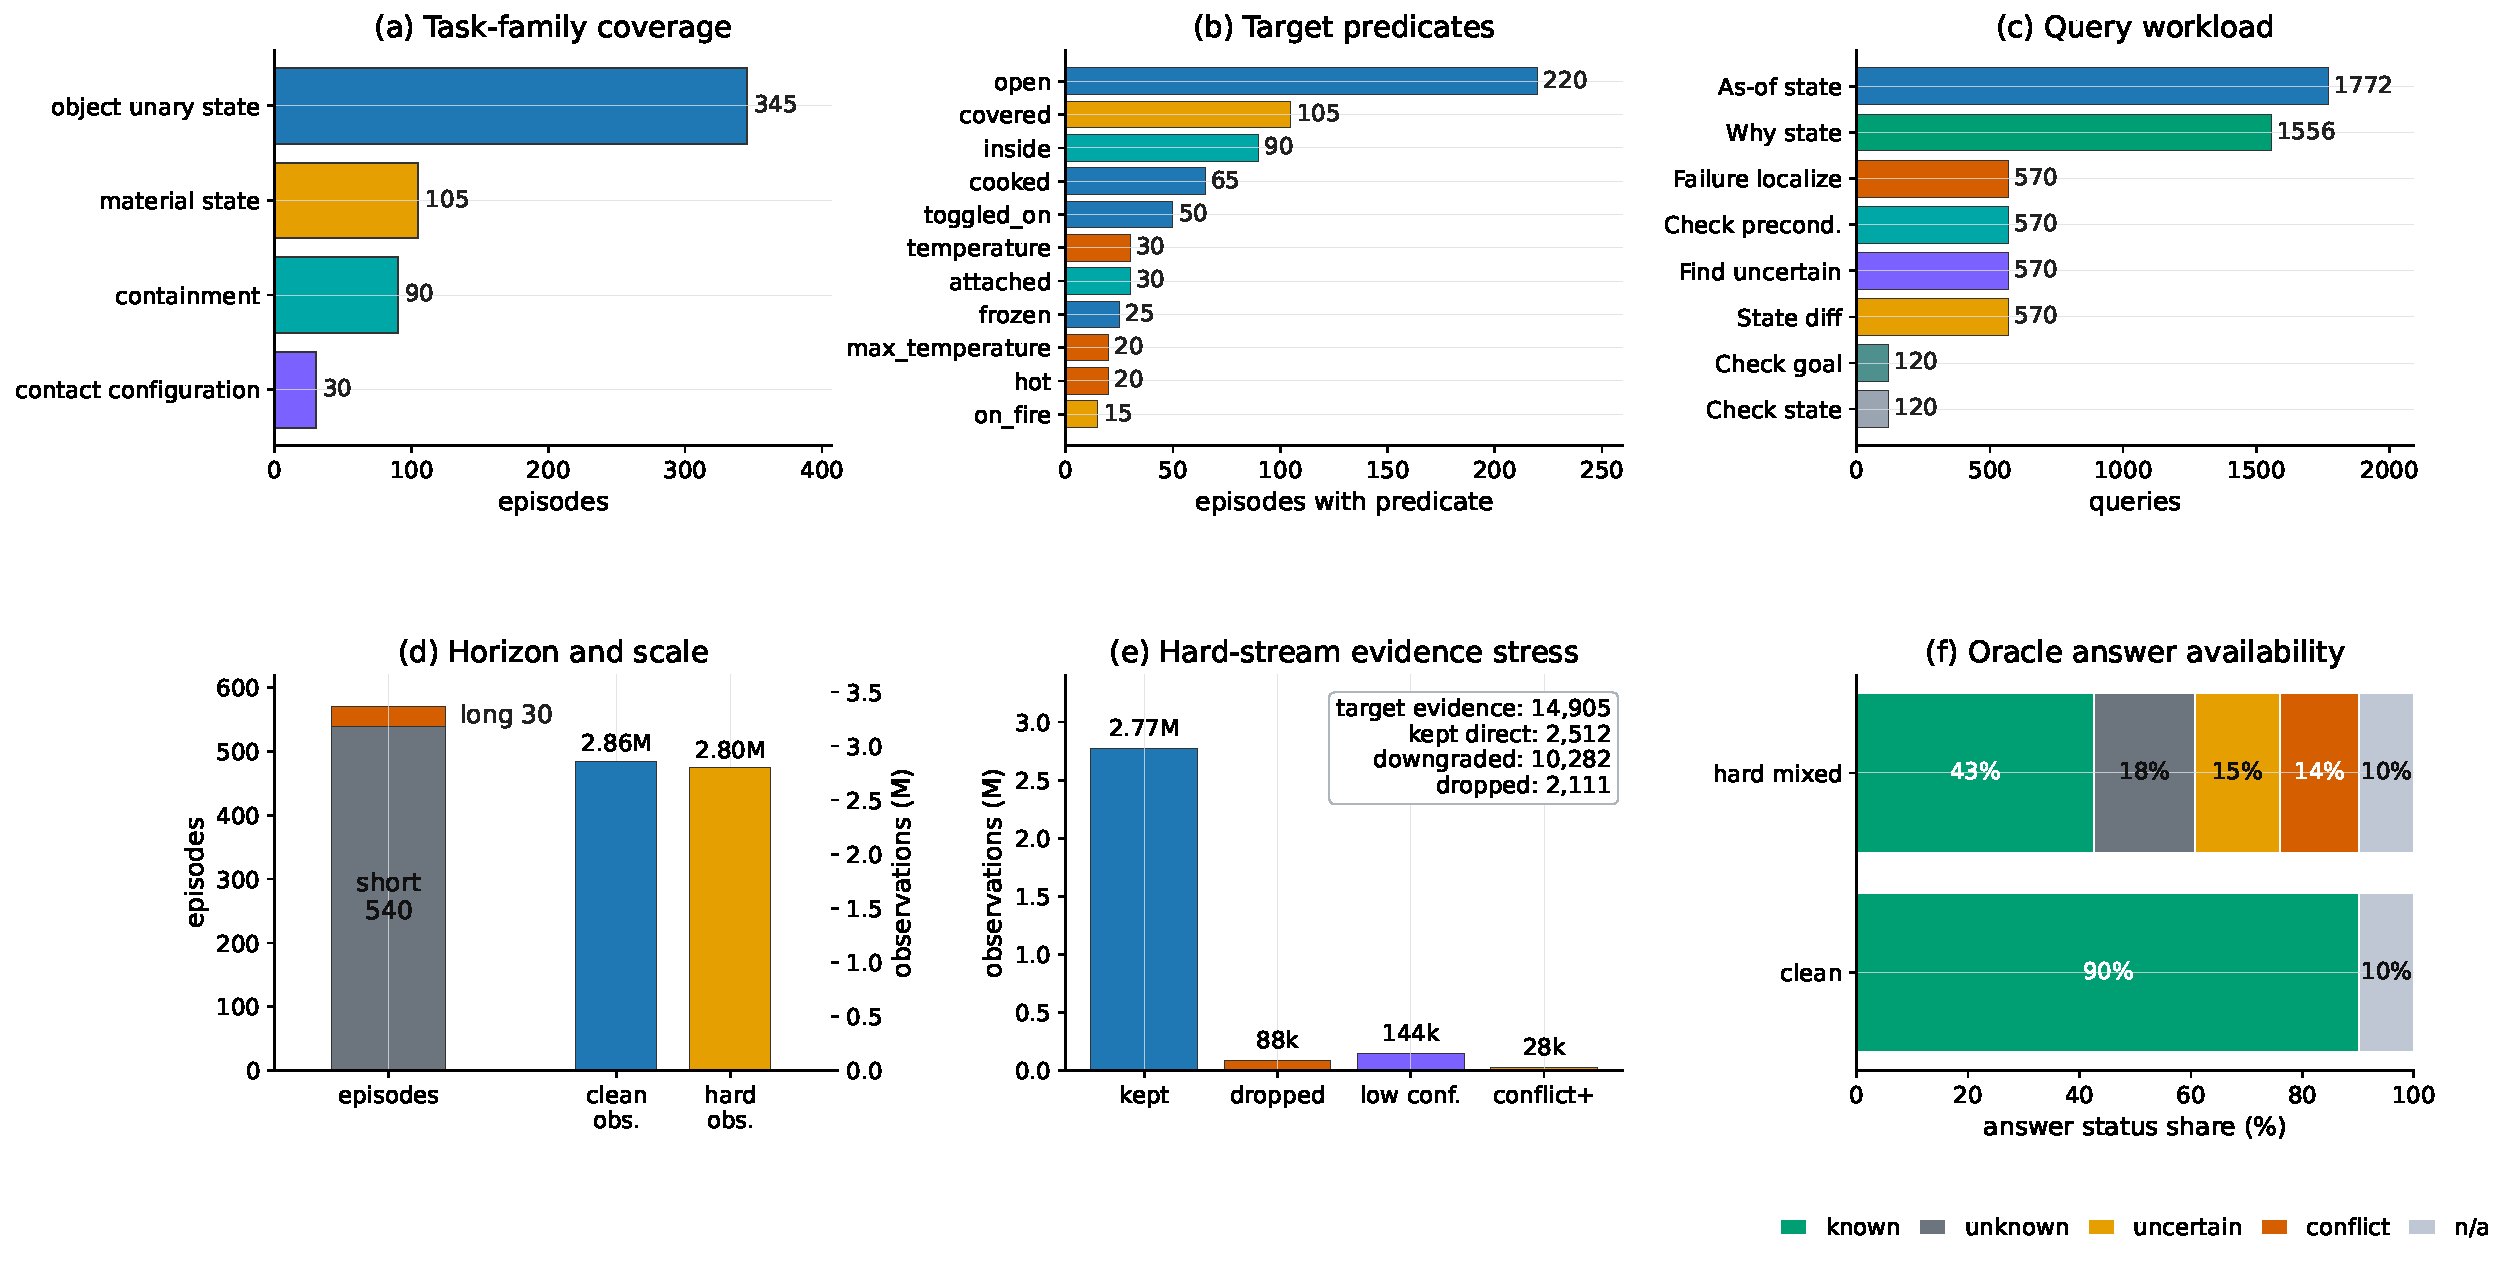
\includegraphics[width=\textwidth]{figures/figA_benchmark_profile.pdf}
\caption{Benchmark artifact profile. \bench\ covers 570 simulator-grounded episodes over 36 activities, four task-state families, and 11 target predicates. The hard mixed stream stresses target evidence and shifts answer availability from mostly known clean answers to a mixture of known, unknown, uncertain, conflicting, and not-applicable answers.}
\label{fig:artifact-profile}
\end{figure*}

\subsection{Artifact Characterization}

The reported artifact supports the first EAB claim: \bench\ is a concrete, validated benchmark package rather than only a proposal. Fig.~\ref{fig:artifact-profile} summarizes the released workload. The artifact contains 570 simulator-grounded episodes, 36 activities, four task-state families, 11 target predicates, 5,848 hard queries, 2.86M clean observations, and 2.80M hard mixed observations. The query set covers point state checks, bitemporal as-of probes, provenance queries, full-episode diffs, uncertainty sets, preconditions, failure localization, and task-goal checks. The target predicates cover object unary state, material state, containment, and contact configuration. This diversity is important because a benchmark limited to one predicate family would be easy to overfit with a specialized rule.

\begin{figure*}[!t]
\centering
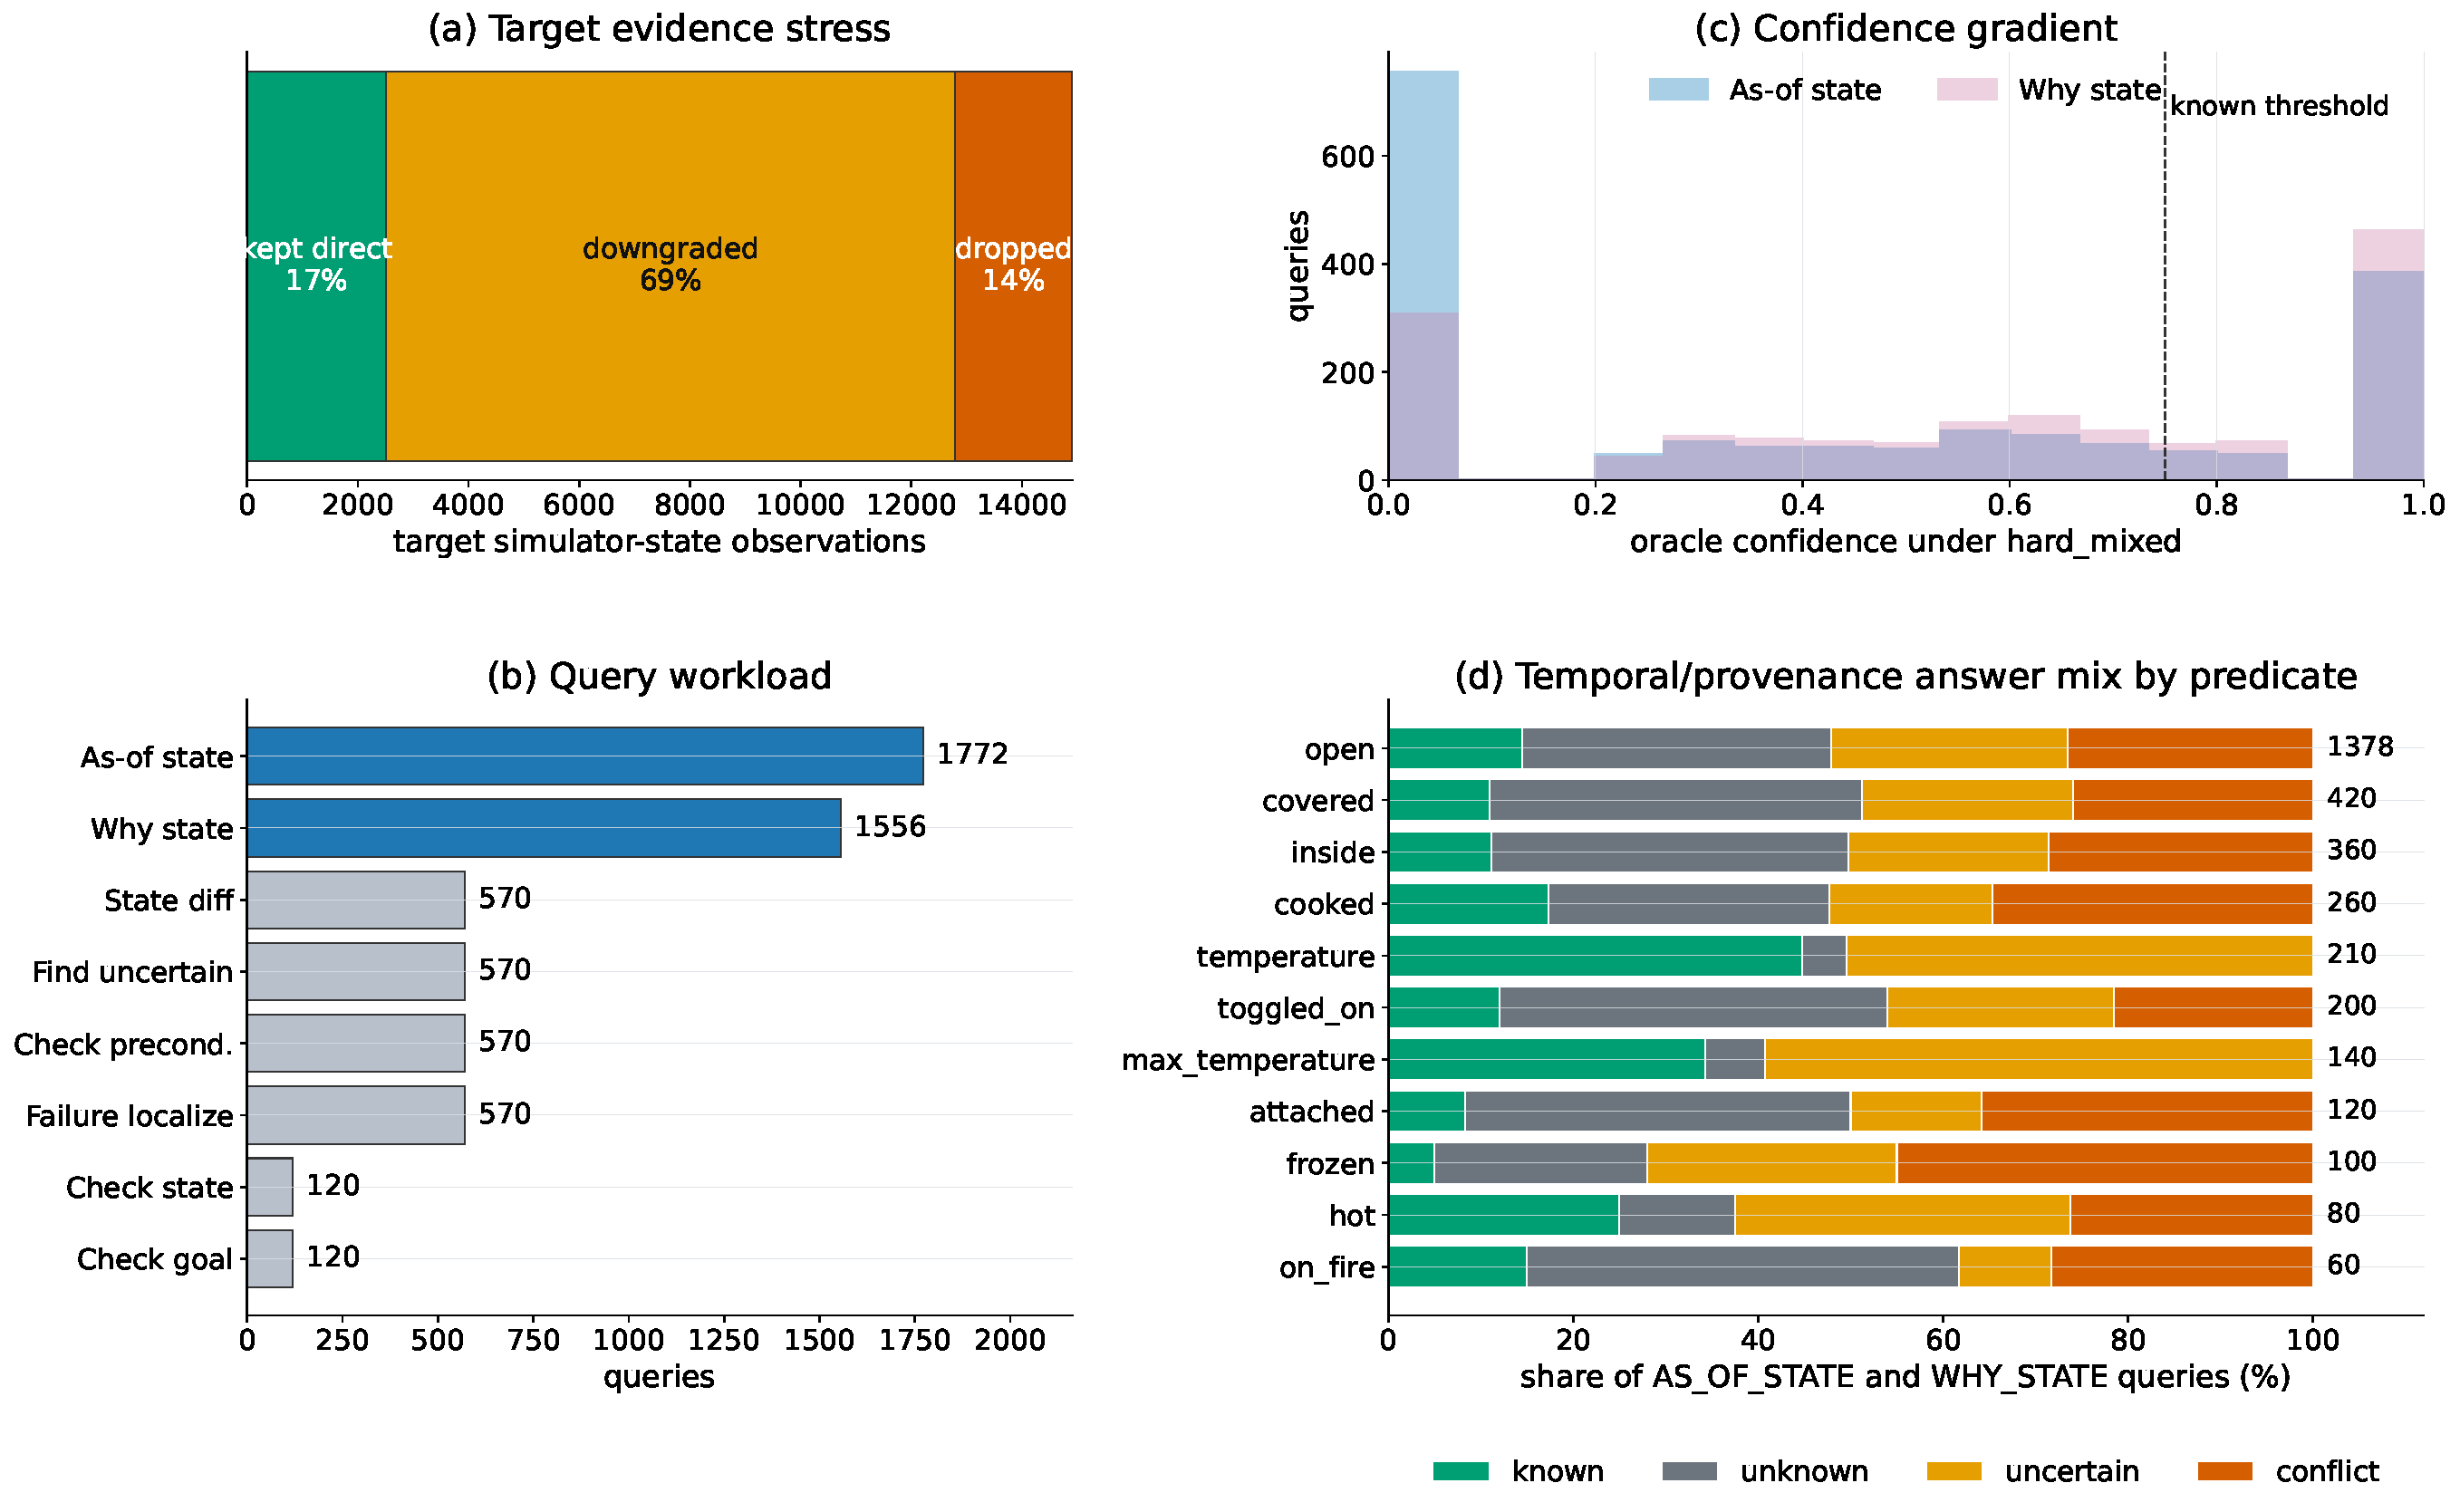
\includegraphics[width=\textwidth]{figures/figB_query_difficulty_matrix.pdf}
\caption{Hard-split mechanism and query difficulty profile. The hard stream keeps only a minority of target simulator-state observations as direct evidence, while downgrading or dropping the rest. The resulting workload emphasizes temporal and provenance queries and produces graded known, unknown, uncertain, and conflicting answer conditions across target predicates.}
\label{fig:hard-profile}
\end{figure*}

\subsection{Hard-Split Difficulty}

Fig.~\ref{fig:hard-profile} explains why the hard split is more than a larger file. Among 14,905 target simulator-state observations, only 2,512 remain as direct target evidence, 10,282 are downgraded to lower-confidence evidence, and 2,111 are dropped. The overall stream also contains 87,571 dropped observations, 144,011 low-confidence observations, and 27,883 injected conflicts. This perturbation is target-aware: it stresses evidence near the states that queries ask about, while leaving most background observations intact.

The hard split is therefore a controlled stress test for data-management behavior. It is not an empirical model of every real sensor failure. Its purpose is to create missing, low-confidence, delayed, and conflicting evidence regimes in which systems must decide whether a state is known, unknown, uncertain, or conflicting. The confidence and predicate panels in Fig.~\ref{fig:hard-profile} show that the resulting workload is not binary. Different predicates exhibit different answer mixtures, and temporal/provenance queries include high-confidence, low-confidence, missing, and conflicting cases.

\subsection{Long State Chains}

Most episodes in the reported artifact are short controlled transitions, but the release also includes a 30-episode long state-chain subset over cooking and freezing activities. The cooking chains move from an actuator state to temperature and maximum-temperature changes, and then to hot and cooked states. The freezing chain moves from opening the refrigerator to temperature change and then to frozen state. This subset is not large enough to claim broad long-horizon BEHAVIOR coverage, but it demonstrates that the benchmark can express multi-stage temporal state maintenance beyond a single target flip.

\begin{figure*}[!t]
\centering
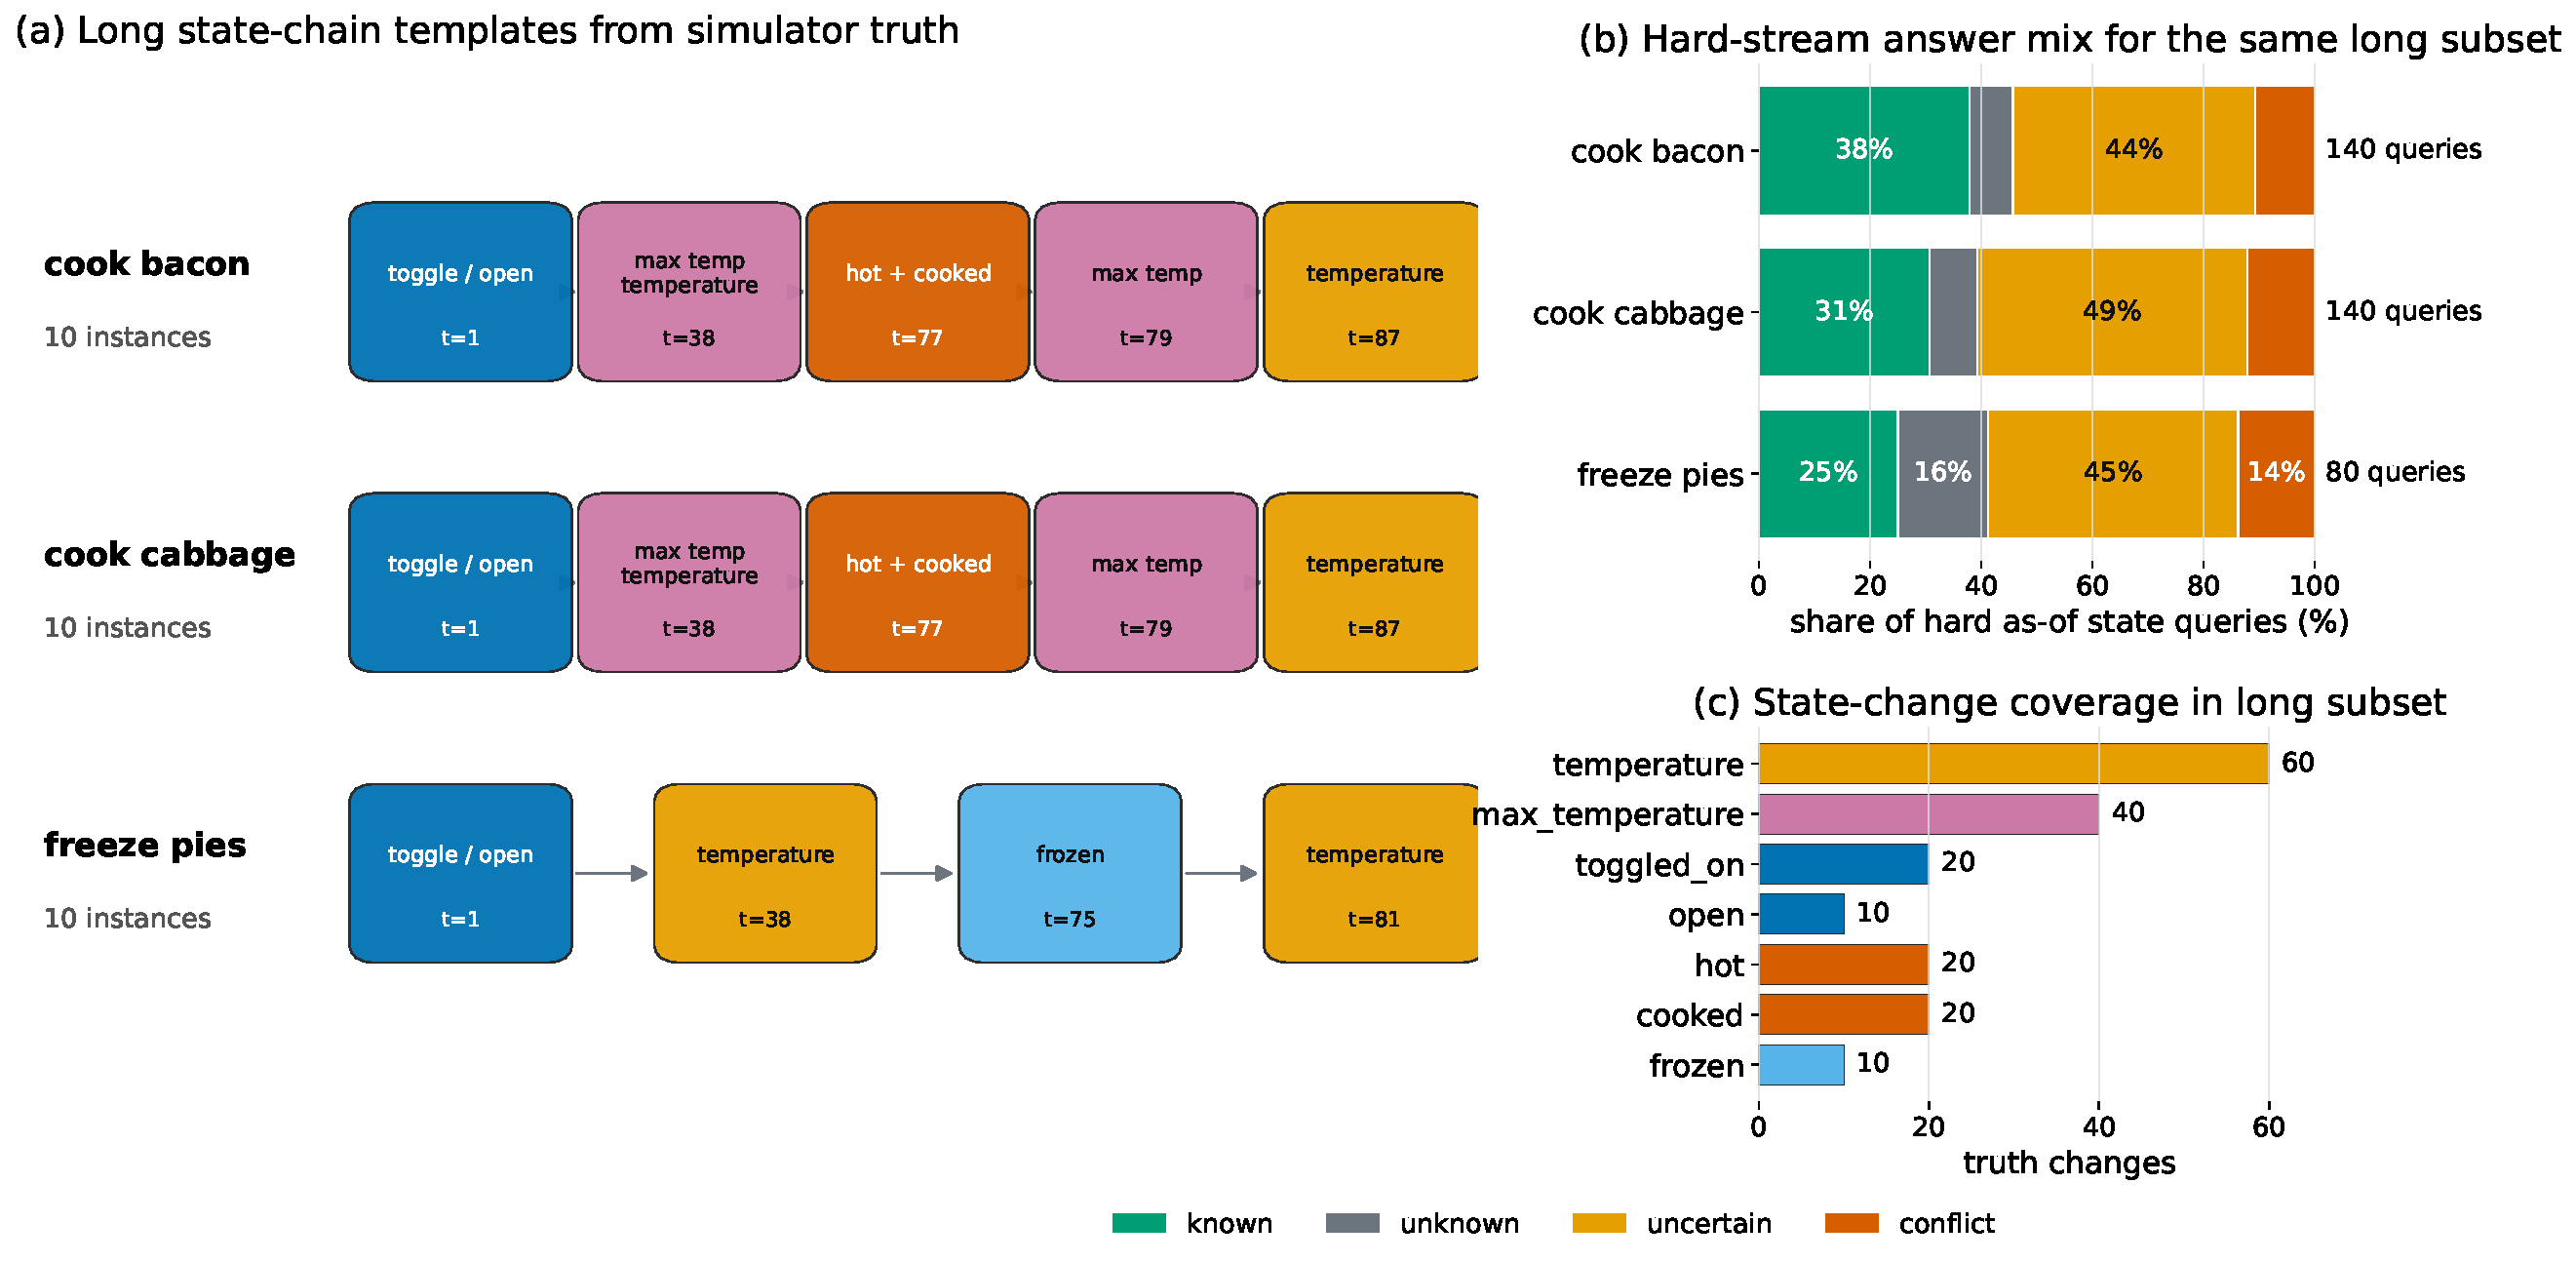
\includegraphics[width=0.84\textwidth]{figures/figC_long_state_chain_timeline.pdf}
\caption{Aggregated long state-chain templates. The 30-episode long subset adds multi-stage temporal maintenance cases, such as actuator, temperature, hot, cooked, and frozen state chains, to the larger short-transition benchmark.}
\label{fig:long-chain}
\end{figure*}

Fig.~\ref{fig:long-chain} makes this diagnostic role explicit. The long subset is small and is not a separate robotics claim; it shows that the artifact can express chained state consequences and convert them into temporal availability cases under hard mixed evidence.

\begin{figure*}[!t]
\centering
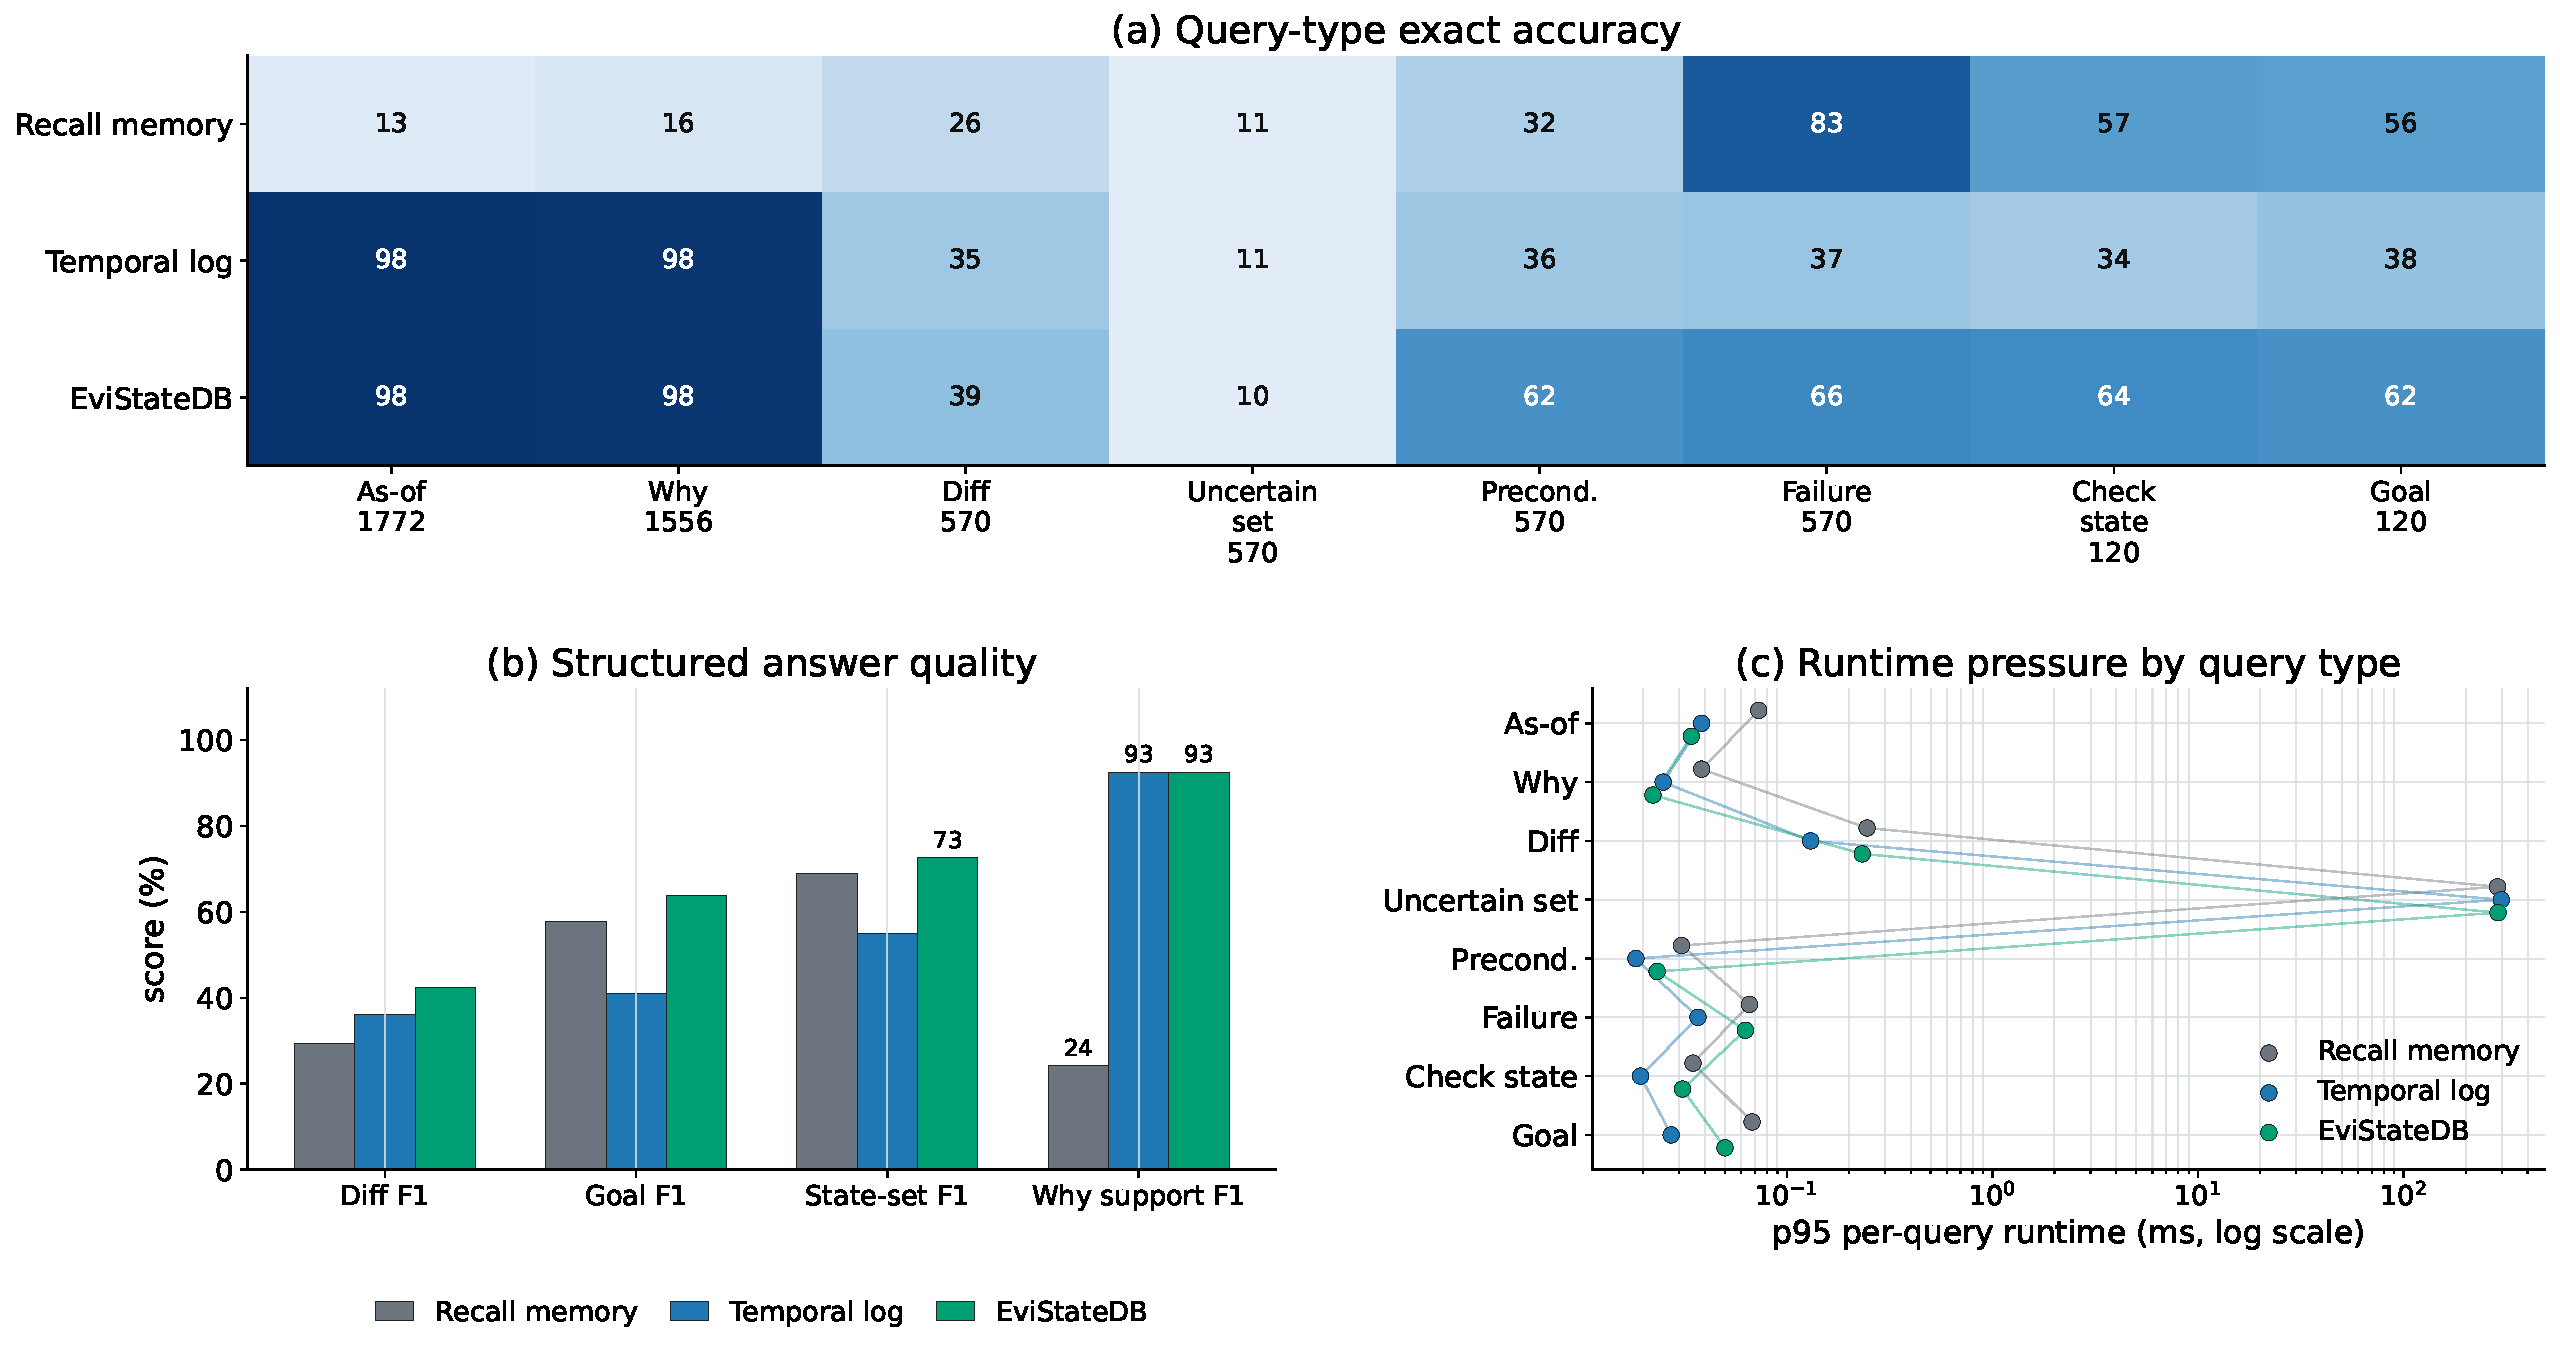
\includegraphics[width=\textwidth]{figures/figD_baseline_main_results.pdf}
\caption{Baseline results on the final hard split. The upper heatmap reports query-type exact accuracy, the lower-left panel reports structured answer metrics, and the lower-right panel reports p95 per-query runtime from prediction outputs. All methods cover the full 5,848-query workload.}
\label{fig:baseline-results}
\end{figure*}

\subsection{Baseline Results}

Fig.~\ref{fig:baseline-results} compares three reference baselines on the final hard split. Recall memory answers from retrieved or recent evidence without maintaining a temporal state view. Temporal log keeps an explicit event log and evaluates temporal queries over it. \engine\ maintains a bitemporal task-state view with support and contradict evidence.

The overall exact accuracies are 25.2\% for Recall memory, 69.0\% for Temporal log, and 75.6\% for \engine. These results support the benchmark's diagnostic goal: the workload separates retrieval-style memory, append-only temporal lookup, and materialized temporal-state views. The largest gap is between retrieval-style memory and the two temporal baselines; the additional gain from Temporal log to \engine\ is smaller and concentrates in structured and task-derived workloads. Temporal log and \engine\ reach 98\% exact accuracy on \texttt{AS\_OF\_STATE} and \texttt{WHY\_STATE}, but they still struggle on structured workloads. \engine\ reaches only 39\% exact accuracy on \texttt{STATE\_DIFF} and 10\% on \texttt{FIND\_UNCERTAIN\_STATES}, although its partial structured metrics are higher: 42.4\% Diff F1, 63.8\% Goal F1, 72.6\% State-set F1, and 92.5\% Why-support F1.

The runtime panel reports per-query prediction time, not full end-to-end indexing or stream-loading time. It shows a different stress point: most point-state queries are inexpensive after indexing, while \texttt{FIND\_UNCERTAIN\_STATES} dominates p95 query time for all methods. This is useful benchmark information because it separates semantic difficulty from query-time pressure.

\subsection{Failure and Difficulty Diagnostics}

The baseline diagnostics separate two different messages. First, answer status matters. Recall memory fails especially on unknown, uncertain, and conflict answers, while Temporal log and \engine\ recover most unknown and uncertain statuses. Second, the high predicate-level accuracy for Temporal log and \engine\ on \texttt{AS\_OF\_STATE} and \texttt{WHY\_STATE} should not be overstated. It means that explicit event-time and transaction-time maintenance is effective for these two query families. It does not mean that all of \bench\ is easy, because the residual errors in Fig.~\ref{fig:baseline-results} concentrate in set-valued uncertainty, state diffs, preconditions, failure localization, and goal views.

\begin{figure*}[!t]
\centering
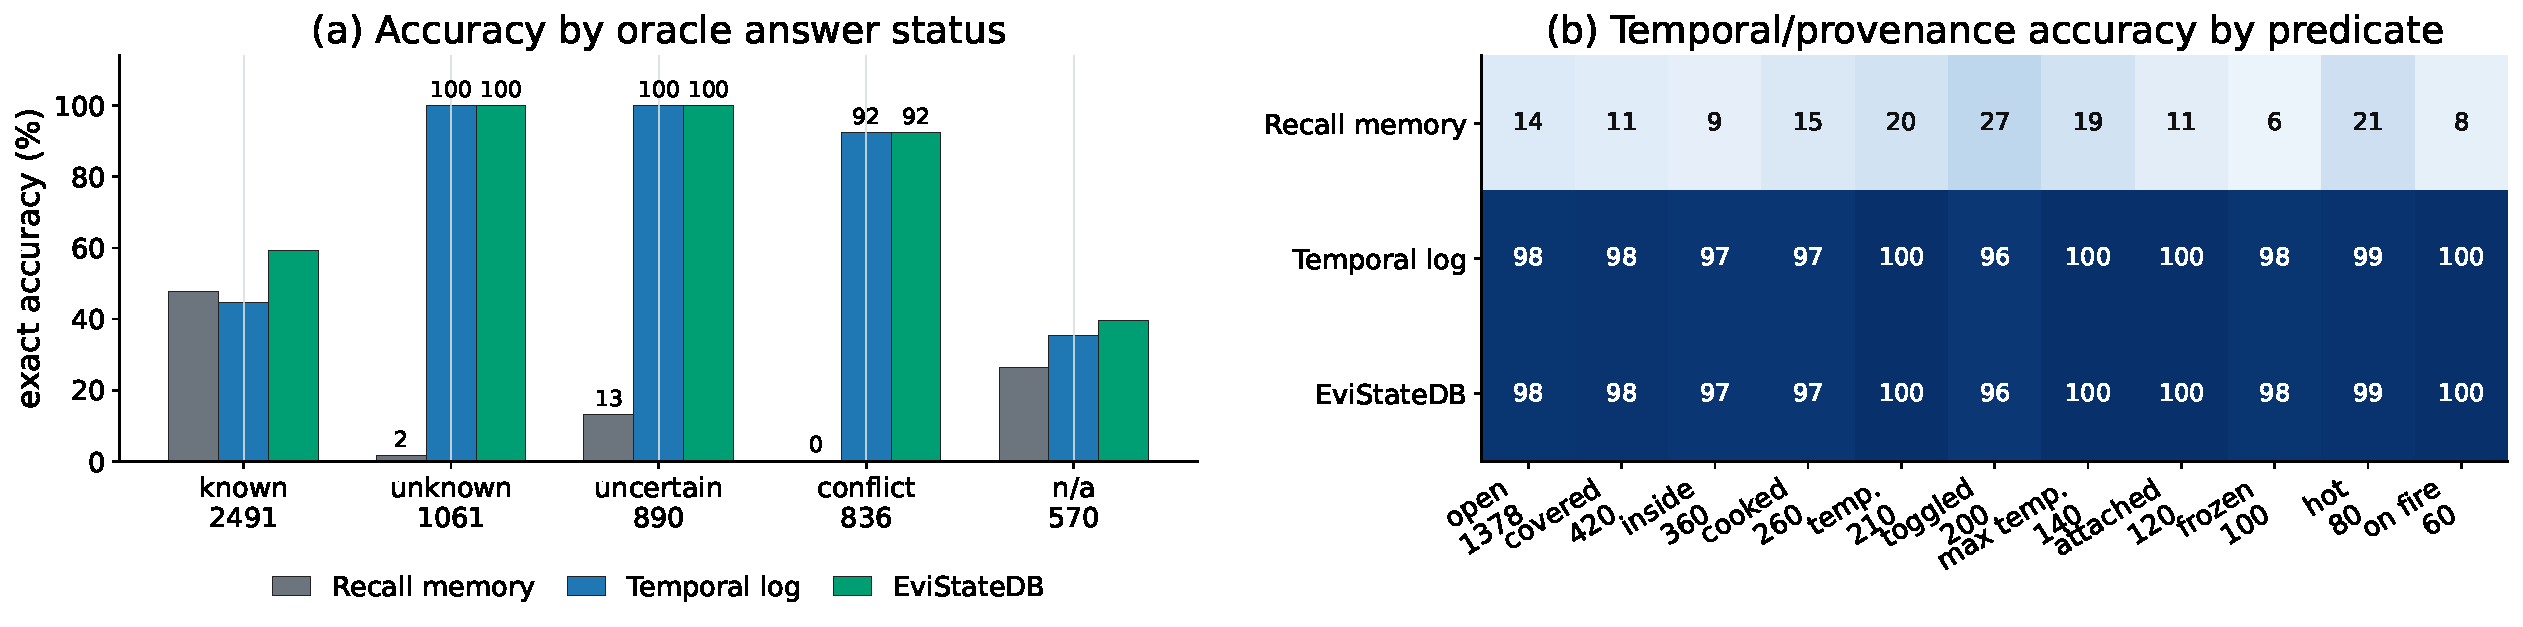
\includegraphics[width=0.84\textwidth]{figures/figE_failure_difficulty_analysis.pdf}
\caption{Difficulty analysis by answer status and predicate. Recall memory degrades across answer statuses and target predicates, while explicit temporal-state baselines largely solve \texttt{AS\_OF\_STATE} and \texttt{WHY\_STATE}.}
\label{fig:failure-diagnostics}
\end{figure*}

Fig.~\ref{fig:failure-diagnostics} explains where residual difficulty comes from. Retrieval fails broadly, while Temporal log and \engine\ largely recover temporal and provenance answers. The remaining difficulty is therefore concentrated in answer shapes that require sets, diffs, preconditions, failure localization, and goal aggregation.

The interpretation should avoid two common mistakes. It should not treat \engine\ as the oracle merely because it is the reference engine. It should also not claim that a lower score means a method is bad for all embodied AI tasks. A retrieval memory that performs poorly on state diffs may still be useful for open-ended question answering. The EAB claim is narrower and more useful: \bench\ identifies which systems are good at temporal task-state view maintenance under a shared, reproducible workload.

\section{Lessons, Limitations, and Artifact Availability}
\label{sec:discussion}

\subsection{Lessons from the Benchmark Design}

\bench\ exposes five practical lessons. First, latest-state memory is not a sufficient abstraction because late evidence can revise as-of answers and contradict evidence can make a state uncertain or conflicting. Second, retrieval and view maintenance answer different questions: retrieval can surface evidence, but task execution often needs a maintained predicate value, change set, or goal view. Third, provenance should be first-class because support and contradict evidence are needed for why queries, failure localization, and trust calibration. Fourth, goal views are not just convenience layers; they can fail even when individual predicates are partly correct. Fifth, validation reports are benchmark artifacts, since malformed query metadata or leaked answer fields can invalidate comparisons as much as model errors.

\subsection{Limitations}

\bench\ makes a controlled isolation choice. The main artifact is simulator-grounded and structured; it does not claim to solve raw perception or low-level robot control. This is a limitation, but also a design requirement for a reproducible data-management benchmark, because folding perception and control into the main score too early would make failures hard to attribute. The reported baseline set is also intentionally conservative: neural memory, LLM-based agents, and full embodied pipelines fit the benchmark only when their public inputs, inference budgets, and output schemas can be made comparable.

\subsection{Artifact Availability}

The benchmark release provides public task specifications, observation streams, query sets, manifests, validation reports, build commands, baseline implementations, prediction schemas, and evaluator scripts. Hidden timelines and answer sets are used for evaluation. The minimal reproduction path builds or validates public artifacts, runs each baseline on the hard mixed stream, validates prediction schema, evaluates predictions, and regenerates the reported tables and figures.

\section{Related Work}
\label{sec:related}

\subsection{Embodied Task and Simulation Benchmarks}

BEHAVIOR introduced a benchmark of everyday household activities with predicate-logic activity specifications and simulation-based evaluation~\cite{srivastava2022behavior}. BEHAVIOR-1K scales this line of work to 1,000 activities and introduces OmniGibson as a simulation environment for realistic physics and rendering~\cite{li2024behavior1k}. Habitat and Habitat 2.0 support embodied navigation and rearrangement evaluation~\cite{savva2019habitat,szot2021habitat}; AI2-THOR provides an interactive 3D environment for visual AI~\cite{kolve2017ai2thor}; VirtualHome represents household activities as executable programs~\cite{puig2018virtualhome}; and TEACh studies embodied agents that interact through dialogue~\cite{padmakumar2022teach}. \bench\ uses the same general idea that task specifications and simulator truth can ground evaluation, but it changes the target from embodied task success to temporal task-state view maintenance.

ALFRED evaluates instruction following~\cite{shridhar2020alfred}, and OpenEQA evaluates embodied question answering over episodic memory and active exploration~\cite{majumdar2024openeqa}. These benchmarks ask whether an agent can act or answer language questions. \bench\ asks whether a system can maintain and query a temporal state view from imperfect evidence, without prescribing the system's internal memory architecture.

\subsection{Temporal, Stream, and Provenance Data Management}

Temporal databases separate the time when a fact is valid in the modeled world from the time when a database records or knows the fact~\cite{snodgrass1999developing,jensen1999temporal}. Stream systems study continuous processing over arriving data~\cite{babcock2002models,garofalakis2016data}. Incremental view maintenance studies how derived database state can be updated after base changes~\cite{gupta1995maintenance,zhuge1995view}. Provenance and uncertain-data systems address evidence and noisy facts~\cite{green2007provenance,cheney2009provenance,aggarwal2009uncertain,dalvi2007efficient}. \bench\ brings these ideas into embodied task-state maintenance, where event-time and arrival-time mismatch, missing observations, conflicting evidence, and task-derived goal views appear together.

\subsection{Experiment, Analysis, and Benchmark Papers}

Database benchmark and EAB papers often contribute workload models, artifact rules, and diagnostic analyses rather than only a new algorithm. LDBC standardizes graph workloads~\cite{erling2015ldbc,iosup2016ldbc}; TSM-Bench benchmarks time-series systems~\cite{khelifati2023tsmbench}; and FinBench defines a financial graph transaction workload~\cite{qi2025finbench}. Recent EAB papers similarly contribute evaluation frameworks and fine-grained diagnostics, including SQLMorph~\cite{malekpour2026sqlmorph}, BEACON~\cite{najafi2025beacon}, and plan-based AQP analysis~\cite{mu2025aqp}. \bench\ follows this pattern: the contribution is the benchmark artifact, workload, evaluator, and analysis of where baseline strategies succeed or fail.

\section{Conclusion}

\bench\ is a data-management benchmark for temporal task-state view maintenance over embodied observation streams. It separates public observation streams and queries from hidden timelines and answers, evaluates systems through standardized QueryAnswers, and makes event time, arrival time, evidence, perturbations, and task-derived state views first-class benchmark concerns. \engine\ provides a reference baseline engine, but the benchmark oracle comes from simulator truth and task specifications. The reported artifact and experiments show that temporal maintenance strategies outperform retrieval-style memory on this workload, while structured, set-valued, and task-derived queries remain open stress points for submitted systems.

\section*{AI-Generated Content Acknowledgement}

The authors used AI-assisted tools during manuscript drafting, code editing, experiment-log summarization, and figure-preparation support. The authors reviewed, edited, and verified the submitted content and remain responsible for the correctness, originality, and integrity of the paper.

\bibliographystyle{IEEEtran}
\bibliography{refs}

\end{document}
